\documentclass[a4paper,11pt]{article}
\usepackage[english]{babel}
\usepackage[utf8]{inputenc} \parindent=1cm \usepackage[pdftex]{graphicx} \usepackage{anysize} \marginsize{2cm}{2cm}{1.5cm}{1.5cm}
\usepackage{multirow}
\begin{document} \title{Methylation in the promoter region of SRD5A genes in patients with different grade of prostate cancer} \author{Sara Jordá, Jesús M. Torres} \maketitle
	\begin{abstract}
		\begin{bf}Repository URL: https://github.com/sarajrcl/proyecto\_final.git \end{bf} \\ 
	
	\begin{bf}Background: \end{bf}Prostate Cancer (PCa) is a cause of public concern in the Western World. Within the prostate, the enzyme steroid 5a-Reductase (5a-R) converts circulating testosterone (T) into dihydrotestosterone (DHT), the primary androgen responsible for the development, maturation and function of the prostate gland and also implicated in the pathogenesis of prostatic diseases. 5a-R occurs as three isozymes, with a controversial role for 5a-R3 in the androgen metabolism and prostate growth. \\
		Currently, there are no prognosis biomarkers for PCa, but the need for personalized treatment for each patient illustrates that the discovery of new markers are becoming increasingly urgent. DNA methylation is an important epigenetic mechanism for gene expression regulation, and plays an essential role in the initiation and progression of tumours, where hypermethylation of critical genes are associated with gene silencing. Thus, this epigenetic mark could be potential biomarker and a target for treating PCa. Epigenetic research uses powerful techniques for the study of DNA methylation, such as sodium bisulfite modification of DNA associated with polymerase-chain-reaction procedures. One of these approaches is the Methylation-Sensitive High Resolution Melting (MS-HRM), a new sensitive and specific method for the detection of methylation. It allows analyzing the methylation status of an unknown sample by comparing its dissociation or melting profile with the melting profiles of methylated and unmethylated DNA controls. \\ \\
		We hypothesized that the methylation status of CpG islands in the promoter region of SRD5A genes may play a role in the development and progression of PCa. The objective of this study is to stablish an optimal workflow using MS-HRM in order to detect changes in the methylation levels of SRD5A1 and SRD5A2 promoters, in normal and malignant prostate tissues from patients with different grade of PCa. \\
		
		\begin{bf} Patients and Methods: \end{bf} We used formalin-fixed paraffin-embe-dded (FFPE) tissue samples from 18 patients with a different grade of PCa (n=9 low-grade PCa; n=9 high-grade PCa). Due to the challenging use of this type of starting material, we stablished an optimal methodology to isolate the DNA with the highest concentration and quality and we optimized the design of primers for a MS-HRM downstream analysis. \\
		\begin{bf}Key words: \end{bf}prostate cancer (PCa); 5a-reductase; DNA methylation; biomarker; Methylation-sensitive high-resolution Melting (MS-HRM).\end{abstract}
	
			
\section{Introduction}
	Prostate Cancer (PCa) is the third most common cause of cancer-related death amongst men in Western countries and its development increases with age. Moreover, it is expected that as life expectancy growths, the number of deaths due to this cancer will be greater \cite{Bashir2015, Thompson2013}. PCa is defined as a clinically highly heterogeneous disease, while most PCa patients have little or inexistent clinical manifestation and a slowly tumour progression, others suffer an aggressive and metastatic cancer with an almost inevitable lethal result \cite{Albertsen2005}. As it is shown in Figure 1, the enzymes responsible of the conversion of T to DHT, which are encoded by the genes SRD5A1 and SRD5A2, are present at different levels in prostate; 5a-R2 is the most abundant isozyme in the prostate cells whereas 5a-R1 represents only the 10\% of the total reductase levels. Nevertheless, during PCa initiation and tumour progression, there is an androgen-dependent inverse transcriptional regulation of these isozymes, SRD5A1 expression increases while the expression of SRD5A2 decreases \cite{Steers2001}.  \\ 

Recent emerging molecular biological technologies help us to know that epigenetic alterations such as DNA methylation within the regulatory (promoter) regions of genes are associated with transcriptional silencing in cancer. Promoter hypermethylation of critical pathway genes could be potential biomarkers and therapeutic targets for prostate cancer \cite{Yang2012}.
In this context, we propose to study possible biomarkers at epigenetic level in SRD5A1 and SRD5A2. Epigenetic modifications consist in heritable and reversible biochemical changes in DNA that affects gene expression without altering the primary DNA sequence. Alterations in the epigenome are signal of PCa and are involved not only in the malignant initiation but also in the tumour progression \cite{Goering2012}. DNA methylation is the most frequently studied epigenetic change in prostate cancer; it is an early event that continues on through the evolution of the cancer. Methylation of CpG islands acts are associated with transcriptional silencing in cancer (Figure 2). Although the mechanisms by which these alterations arise in PCa are not cleared, the fact that they occur at a much higher frequency than mutations, shows the potential of these methylation signatures to be used as biomarkers for diagnostic, prognostic and treatment response of this type of cancer \cite{Strand2014, Yang2012}  \\ \\ Given the above background, we are interested in assess possible methylation changes in the promoter region of SRD5A genes, throughout PCa evolution. We hypothesized that the methylation status of CGIs in the promoter region may play a role in the development and progression of PCa. 

\section{State of the art}

Currently, the hypermethylation of over 40 genes with functions that include tumor suppressor, tumor metastasis, metabolism and DNA repair, have been investigated for their potential role in PCa \cite{Steers2001}. Nevertheless, little is known about the DNA methylation within the regulatory region of SRD5A genes and its involvement in PCa. In this study, we suggest that methylation changes in the CGIs of the SRD5A2 promoter region might be occurring in patients with PCa and throughout the progression of the disease. \\ Epigenetic research uses powerful techniques for the study of DNA methylation, such as sodium bisulfite modification associated with polymerase-chain-reaction procedures \cite{Jeronimo2011}. One of these is the Methylation-Sensitive High Resolution Melting (MS-HRM), a new sensitive and specific method for the detection of methylation. It allows to analyze the methylation status of an unknown sample by comparing its dissociation or melting profile with the melting profiles of methylated and unmethylated DNA controls \cite{Wojdacz2007, Wojdacz2010}. 

\section{Images and tables}
In the images below are shown the synthesis pathway of DHT in the a prostate gland and the effect of the DNA methylation on the gene expression of the cells. The table contains information about the primers used in our MS-HRM analysis with PCa patients samples.

\begin{figure}[h!]

	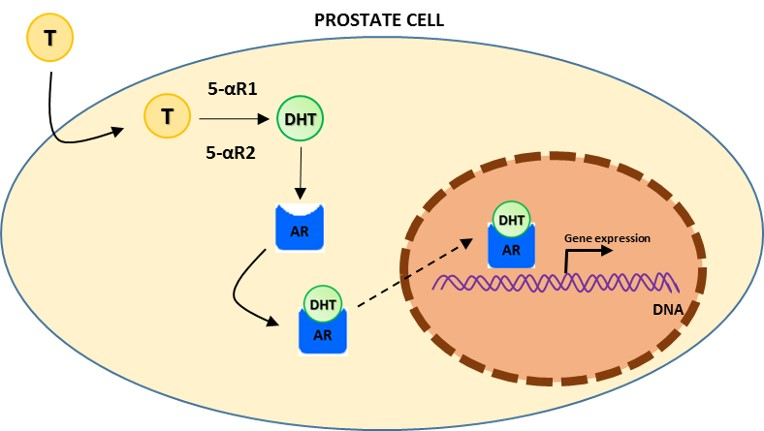
\includegraphics[scale=0.6]{Imagen_DHT}
	\caption{DHT synthesis in the prostate gland.} \label{Imagen_DHT} 
	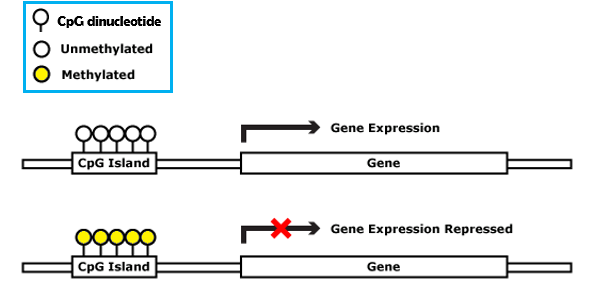
\includegraphics[scale=0.9]{Imagen_DNAmeth}
	\caption{DNA methylation on CpG sites and gene expression.} \label{Imagen_DNAmeth} 

 \end{figure} 


\begin{center} 
	\begin{tabular}{|c|c|c|c|}
	\hline
	Assay name & Primer sequences & T (ºC)  & Amplicon lenght (bp) \\
	\hline SRD5A1.1 & GACGTTTATTTCGAGGTTTAAGGAG & 57,5 & 127 \\
	\hline SRD5A1.2 & TGCATCGATCCGATATAGGGGCTATA & 59 & 132 \\ 
	\hline SRD5A1.3 & CAGTGACCCGTAGCGCGTATTCGACGT & 59,5 & 130 \\
	\hline SRD5A2.1 & ACCGCTAGCAGTCGATCGATCGATG & 60 & 150 \\
	\hline SRD5A2.2 & GTAGCCCAGTCGACGATTGGCTGAG & 59 & 125 \\
	\hline SRD5A2.3 & AGGCTTGGATCGTAGTTATTCGACGT & 58 & 115 \\
	\hline SRD5A2.4 & GAGAGCTAGACTGATCGGATGGGC & 61 & 165 \\
	\hline
	
	\end{tabular}
\end{center}

\section{Formula}
According to the number of nucleotides of the primer sequence, a different Tm calculation is used. 

For sequences \begin{bf} less than 14 nucleotides \end{bf}, the formula is:

$Tm= (n  A+nT) * 2 + (nG+nC) * 4$
\\ For sequences \begin{bf} longer than 13 nucleotides \end{bf}, the equation used is:

$Tm= 64.9 + 41*(nG+C-16.4)/(nA+nT+nG+nC)$
where A,T,G,C are the nitrogenous bases adenine, thymine, guanine and cytosine in the sequence (see \cite{Marmur1962}).


\section{References}

\bibliography{proyecto_final_bibl} \bibliographystyle{unsrt}

\end{document}